\documentclass{standalone}
\usepackage{tikz}
\usetikzlibrary{patterns, positioning}

\begin{document}
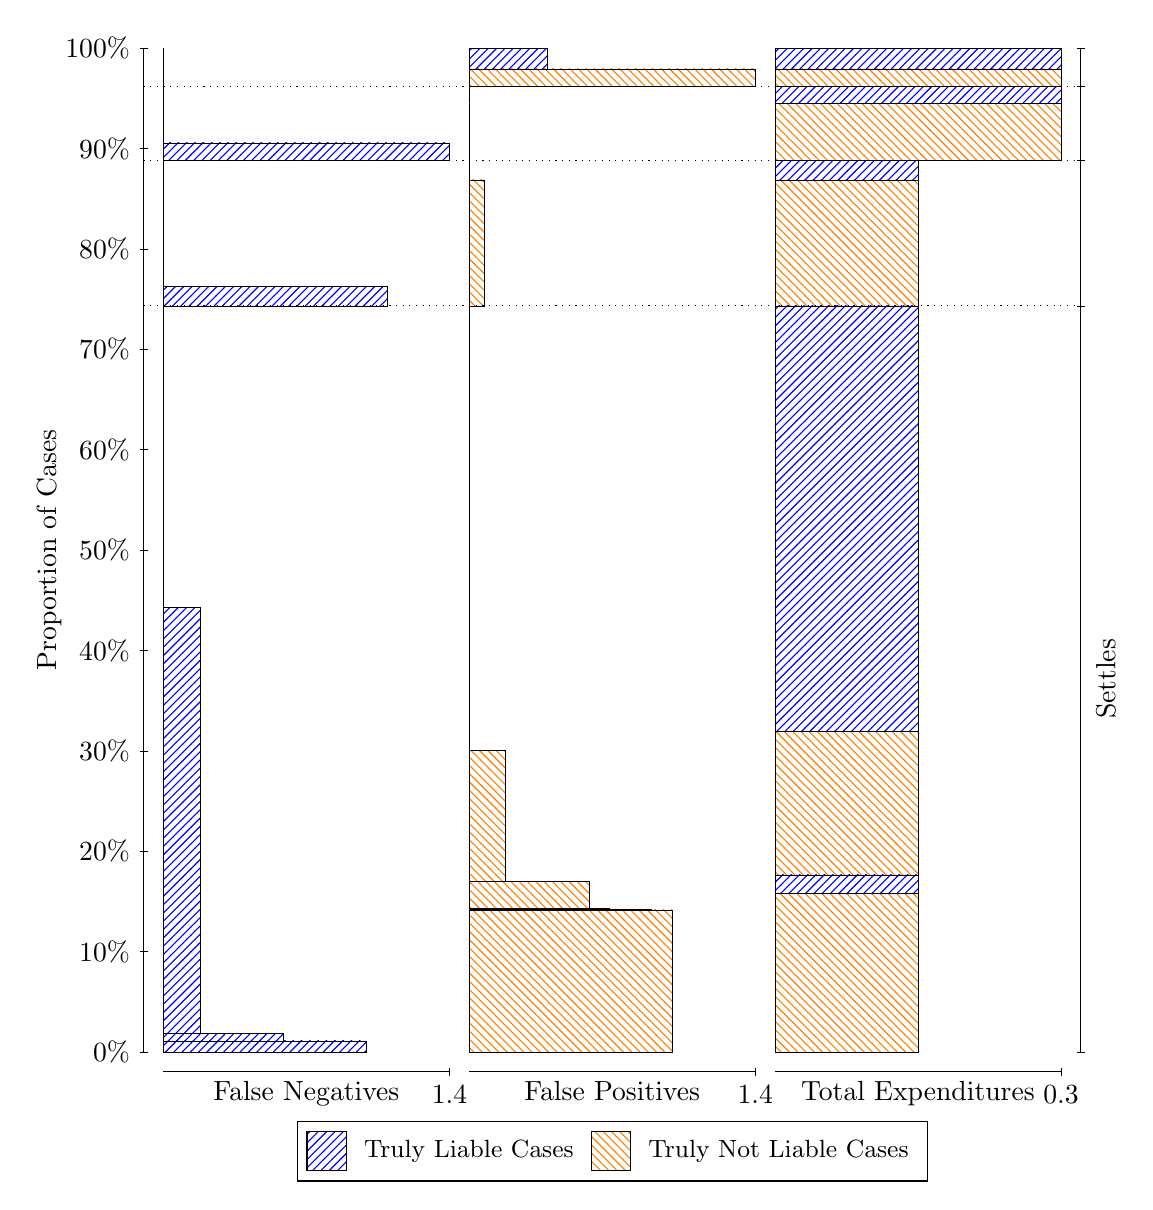
\begin{tikzpicture}
\draw[black, very thin] (1.5,1.75) -- (1.5,14.5);
\node[rotate=90, anchor=center] at (0.3, 8.125) {Proportion of Cases};
\draw[black, very thin] (1.45,1.75) -- (1.55,1.75);
\node[anchor=east] at (1.45, 1.75) {0\%};
\draw[black, very thin] (1.45,3.025) -- (1.55,3.025);
\node[anchor=east] at (1.45, 3.025) {10\%};
\draw[black, very thin] (1.45,4.3) -- (1.55,4.3);
\node[anchor=east] at (1.45, 4.3) {20\%};
\draw[black, very thin] (1.45,5.575) -- (1.55,5.575);
\node[anchor=east] at (1.45, 5.575) {30\%};
\draw[black, very thin] (1.45,6.85) -- (1.55,6.85);
\node[anchor=east] at (1.45, 6.85) {40\%};
\draw[black, very thin] (1.45,8.125) -- (1.55,8.125);
\node[anchor=east] at (1.45, 8.125) {50\%};
\draw[black, very thin] (1.45,9.4) -- (1.55,9.4);
\node[anchor=east] at (1.45, 9.4) {60\%};
\draw[black, very thin] (1.45,10.675) -- (1.55,10.675);
\node[anchor=east] at (1.45, 10.675) {70\%};
\draw[black, very thin] (1.45,11.95) -- (1.55,11.95);
\node[anchor=east] at (1.45, 11.95) {80\%};
\draw[black, very thin] (1.45,13.225) -- (1.55,13.225);
\node[anchor=east] at (1.45, 13.225) {90\%};
\draw[black, very thin] (1.45,14.5) -- (1.55,14.5);
\node[anchor=east] at (1.45, 14.5) {100\%};

\draw[black, very thin] (13.4,1.75) -- (13.4,14.5);
\draw[black, very thin] (13.35,1.75) -- (13.45,1.75);
\node[anchor=west] at (13.35, 1.75) {};
\draw[black, very thin] (13.35,11.226) -- (13.45,11.226);
\node[anchor=west] at (13.35, 11.226) {};
\draw[black, very thin] (13.35,13.072) -- (13.45,13.072);
\node[anchor=west] at (13.35, 13.072) {};
\draw[black, very thin] (13.35,14.016) -- (13.45,14.016);
\node[anchor=west] at (13.35, 14.016) {};
\draw[black, very thin] (13.35,14.5) -- (13.45,14.5);
\node[anchor=west] at (13.35, 14.5) {};

\draw[black, very thin, pattern color=blue, pattern=north east lines] (1.75,1.75) rectangle (4.3264,1.8922);
\draw[black, very thin, pattern color=blue, pattern=north east lines] (1.75,1.8922) rectangle (3.2694,1.9868);
\draw[black, very thin, pattern color=blue, pattern=north east lines] (1.75,1.9868) rectangle (3.0052,1.9879);
\draw[black, very thin, pattern color=blue, pattern=north east lines] (1.75,1.9879) rectangle (2.7409,1.9892);
\draw[black, very thin, pattern color=blue, pattern=north east lines] (1.75,1.9892) rectangle (2.4767,1.9905);
\draw[black, very thin, pattern color=blue, pattern=north east lines] (1.75,1.9905) rectangle (2.2124,7.3927);
\draw[black, very thin, pattern color=orange, pattern=north west lines] (1.75,7.3927) rectangle (1.75,11.226);
\draw[black, very thin, pattern color=blue, pattern=north east lines] (1.75,11.226) rectangle (4.5906,11.472);
\draw[black, very thin, pattern color=orange, pattern=north west lines] (1.75,11.472) rectangle (1.75,13.072);
\draw[black, very thin, pattern color=blue, pattern=north east lines] (1.75,13.072) rectangle (5.3833,13.294);
\draw[black, very thin, pattern color=orange, pattern=north west lines] (1.75,13.294) rectangle (1.75,14.016);
\draw[black, very thin, pattern color=orange, pattern=north west lines] (1.75,14.016) rectangle (1.75,14.236);
\draw[black, very thin, pattern color=blue, pattern=north east lines] (1.75,14.236) rectangle (1.75,14.5);
\draw[black, very thin, pattern color=orange, pattern=north west lines] (5.6333,1.75) rectangle (8.2097,3.5559);
\draw[black, very thin, pattern color=orange, pattern=north west lines] (5.6333,3.5559) rectangle (7.9455,3.5607);
\draw[black, very thin, pattern color=orange, pattern=north west lines] (5.6333,3.5607) rectangle (7.6812,3.5653);
\draw[black, very thin, pattern color=orange, pattern=north west lines] (5.6333,3.5653) rectangle (7.417,3.5697);
\draw[black, very thin, pattern color=orange, pattern=north west lines] (5.6333,3.5697) rectangle (7.1527,3.9192);
\draw[black, very thin, pattern color=orange, pattern=north west lines] (5.6333,3.9192) rectangle (6.0958,5.5832);
\draw[black, very thin, pattern color=blue, pattern=north east lines] (5.6333,5.5832) rectangle (5.6333,11.226);
\draw[black, very thin, pattern color=orange, pattern=north west lines] (5.6333,11.226) rectangle (5.8315,12.826);
\draw[black, very thin, pattern color=blue, pattern=north east lines] (5.6333,12.826) rectangle (5.6333,13.072);
\draw[black, very thin, pattern color=orange, pattern=north west lines] (5.6333,13.072) rectangle (5.6333,13.794);
\draw[black, very thin, pattern color=blue, pattern=north east lines] (5.6333,13.794) rectangle (5.6333,14.016);
\draw[black, very thin, pattern color=orange, pattern=north west lines] (5.6333,14.016) rectangle (9.2667,14.236);
\draw[black, very thin, pattern color=blue, pattern=north east lines] (5.6333,14.236) rectangle (6.6242,14.5);
\draw[black, very thin, pattern color=orange, pattern=north west lines] (9.5167,1.75) rectangle (11.333,3.7636);
\draw[black, very thin, pattern color=blue, pattern=north east lines] (9.5167,3.7636) rectangle (11.333,4.0003);
\draw[black, very thin, pattern color=orange, pattern=north west lines] (9.5167,4.0003) rectangle (11.333,5.82);
\draw[black, very thin, pattern color=blue, pattern=north east lines] (9.5167,5.82) rectangle (11.333,11.226);
\draw[black, very thin, pattern color=orange, pattern=north west lines] (9.5167,11.226) rectangle (11.333,12.826);
\draw[black, very thin, pattern color=blue, pattern=north east lines] (9.5167,12.826) rectangle (11.333,13.072);
\draw[black, very thin, pattern color=orange, pattern=north west lines] (9.5167,13.072) rectangle (13.15,13.794);
\draw[black, very thin, pattern color=blue, pattern=north east lines] (9.5167,13.794) rectangle (13.15,14.016);
\draw[black, very thin, pattern color=orange, pattern=north west lines] (9.5167,14.016) rectangle (13.15,14.236);
\draw[black, very thin, pattern color=blue, pattern=north east lines] (9.5167,14.236) rectangle (13.15,14.5);
\draw[black, dotted] (1.5,11.226) -- (13.4,11.226);
\draw[black, dotted] (1.5,13.072) -- (13.4,13.072);
\draw[black, dotted] (1.5,14.016) -- (13.4,14.016);
\draw[black, very thin] (1.75,1.5) -- (5.3833,1.5);
\node[anchor=north] at (3.5667, 1.5) {False Negatives};
\draw[black, very thin] (5.3833,1.45) -- (5.3833,1.55);
\node[anchor=north] at (5.3833, 1.45) {1.4};

\draw[black, very thin] (5.6333,1.5) -- (9.2667,1.5);
\node[anchor=north] at (7.45, 1.5) {False Positives};
\draw[black, very thin] (9.2667,1.45) -- (9.2667,1.55);
\node[anchor=north] at (9.2667, 1.45) {1.4};

\draw[black, very thin] (9.5167,1.5) -- (13.15,1.5);
\node[anchor=north] at (11.333, 1.5) {Total Expenditures};
\draw[black, very thin] (13.15,1.45) -- (13.15,1.55);
\node[anchor=north] at (13.15, 1.45) {0.3};

\node[black, centered, rotate=90] at (13.72, 6.4879) {Settles};




\draw (7.449999999999999,1.5) node[draw=none] (baseCoordinate) {};
\begin{scope}[align=center]
        \matrix[scale=0.5, draw=black, below=0.5cm of baseCoordinate, nodes={draw}, column sep=0.1cm]{
            \node[rectangle, draw, minimum width=0.5cm, minimum height=0.5cm, pattern=north east lines, pattern color=blue] {}; &
            \node[draw=none, font=\small] (B) {Truly Liable Cases}; &
            \node[rectangle, draw, minimum width=0.5cm, minimum height=0.5cm, pattern=north west lines, pattern color=orange] {}; &
            \node[draw=none, font=\small] (B) {Truly Not Liable Cases}; \\
            };
\end{scope}

\end{tikzpicture}
\end{document}